\documentclass[border=10pt]{standalone}

% --- packages (mirror these in figure.meta.json "requires") ---
\usepackage{tikz}
\usepackage{amsmath}
\usetikzlibrary{positioning, arrows.meta, decorations.pathreplacing, calc}

% --- palette (canonical source: reference/color-palettes/color-palettes.md; light variant) ---
\definecolor{otblue}{HTML}{0072B2}
\definecolor{otorange}{HTML}{E69F00}
\definecolor{otteal}{HTML}{009E73}
\definecolor{otpurple}{HTML}{CC79A7}
\definecolor{otgray}{HTML}{5A5A5A}
\definecolor{otvermillion}{HTML}{D55E00}  % Okabe-Ito vermillion — the "Outer Loop" red (kept color-blind-safe)

\begin{document}
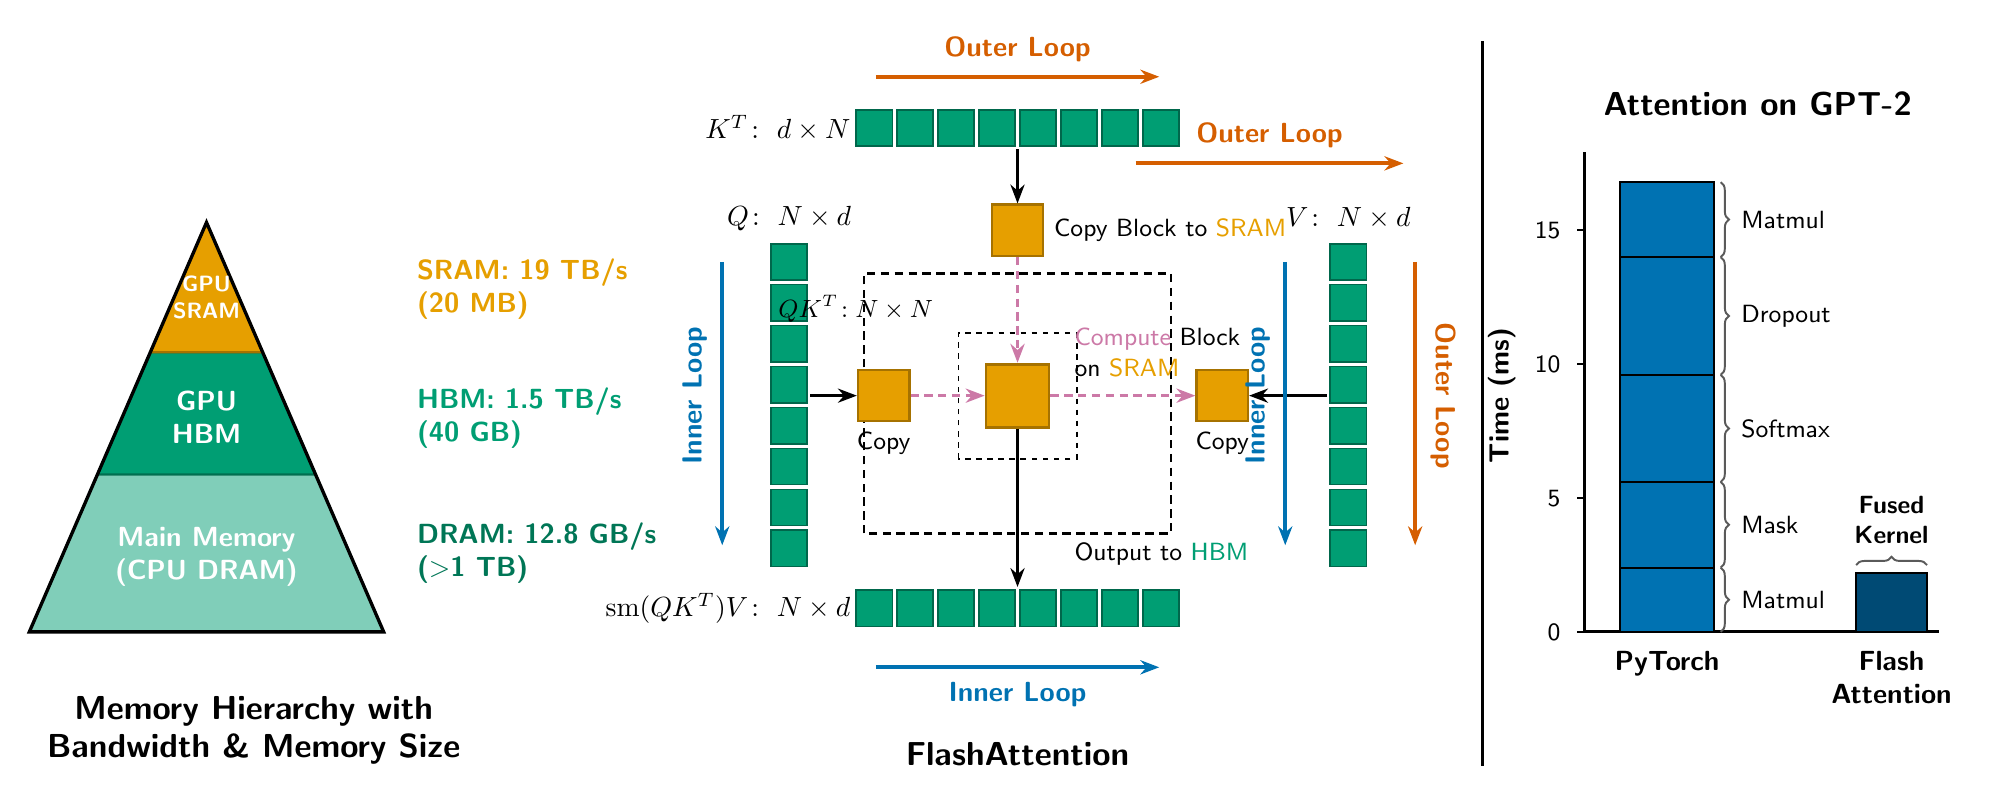
\begin{tikzpicture}[
    >={Stealth[length=2.4mm]},
    font=\sffamily,
    % --- shared element styles -------------------------------------------------
    cell/.style={                                    % a single matrix entry (green)
      draw=otteal!65!black, fill=otteal, line width=0.6pt,
      minimum size=4.6mm, inner sep=0pt},
    copy/.style={                                    % orange "Copy" block in SRAM
      draw=otorange!72!black, fill=otorange, line width=0.9pt,
      minimum size=6.5mm, inner sep=0pt},
    compute/.style={                                 % orange "Compute" block in SRAM
      draw=otorange!72!black, fill=otorange, line width=1pt,
      minimum size=8mm, inner sep=0pt},
    outer/.style={->, draw=otvermillion, line width=1.5pt},   % outer loop (red)
    inner/.style={->, draw=otblue, line width=1.5pt},         % inner loop (blue)
    qkt/.style={->, draw=otpurple, line width=1.2pt, dash pattern=on 3pt off 2pt}, % QK^T flow
    flow/.style={->, draw=black, line width=1pt},             % HBM<->SRAM data move
    matlabel/.style={font=\sffamily\bfseries, text=black},    % matrix name labels
    olabel/.style={font=\sffamily\bfseries, text=otvermillion},
    ilabel/.style={font=\sffamily\bfseries, text=otblue},
    note/.style={font=\sffamily\small, text=black},
    paneltitle/.style={font=\sffamily\bfseries\large, text=black},
  ]

  % =====================================================================
  % PANEL 1 — Memory hierarchy triangle
  % bands of an isoceles triangle: SRAM (orange apex) / HBM (green) / DRAM (teal base)
  % =====================================================================
  \def\Tx{2.0}        % triangle centre x
  \def\Tb{2.25}       % base half-width
  \def\Th{5.2}        % height
  % band heights and half-widths (hw = Tb*(1 - y/Th))
  \def\ya{2.00} \def\hwa{1.385}   % DRAM/HBM boundary
  \def\yb{3.55} \def\hwb{0.714}   % HBM/SRAM boundary

  % DRAM band (light teal)
  \filldraw[draw=otteal!55!black, fill=otteal!50, line width=0.8pt]
    ($(\Tx,0)+(-\Tb,0)$) -- ($(\Tx,0)+(\Tb,0)$)
    -- ($(\Tx,\ya)+(\hwa,0)$) -- ($(\Tx,\ya)+(-\hwa,0)$) -- cycle;
  % HBM band (green)
  \filldraw[draw=otteal!70!black, fill=otteal, line width=0.8pt]
    ($(\Tx,\ya)+(-\hwa,0)$) -- ($(\Tx,\ya)+(\hwa,0)$)
    -- ($(\Tx,\yb)+(\hwb,0)$) -- ($(\Tx,\yb)+(-\hwb,0)$) -- cycle;
  % SRAM apex (orange)
  \filldraw[draw=otorange!72!black, fill=otorange, line width=0.8pt]
    ($(\Tx,\yb)+(-\hwb,0)$) -- ($(\Tx,\yb)+(\hwb,0)$) -- (\Tx,\Th) -- cycle;
  % outline
  \draw[line width=1.2pt] (\Tx-\Tb,0) -- (\Tx+\Tb,0) -- (\Tx,\Th) -- cycle;

  % in-triangle labels (white)
  \node[font=\sffamily\bfseries\footnotesize, text=white, align=center] at (\Tx,4.25) {GPU\\SRAM};
  \node[font=\sffamily\bfseries, text=white, align=center] at (\Tx,2.72) {GPU\\HBM};
  \node[font=\sffamily\bfseries, text=white, align=center] at (\Tx,0.95) {Main Memory\\(CPU DRAM)};

  % right-hand bandwidth / size labels (colored to match the band)
  \node[font=\sffamily\bfseries, text=otorange, anchor=west, align=left] at (\Tx+\Tb+0.3,4.35)
    {SRAM: 19 TB/s\\(20 MB)};
  \node[font=\sffamily\bfseries, text=otteal,  anchor=west, align=left] at (\Tx+\Tb+0.3,2.72)
    {HBM: 1.5 TB/s\\(40 GB)};
  \node[font=\sffamily\bfseries, text=otteal!75!black, anchor=west, align=left] at (\Tx+\Tb+0.3,1.0)
    {DRAM: 12.8 GB/s\\($>$1 TB)};

  % panel title
  \node[paneltitle, align=center] at (\Tx+0.6,-1.25)
    {Memory Hierarchy with\\Bandwidth \& Memory Size};

  % =====================================================================
  % PANEL 2 — FlashAttention dataflow
  % =====================================================================
  \def\Cx{12.3}       % compute / centre column x
  \def\Qx{9.4}        % Q column x
  \def\Vx{16.5}       % V column x
  \def\Qcx{10.6}      % Q copy block x
  \def\Vcx{14.9}      % V copy block x
  \def\topY{6.4}      % K^T row y
  \def\colTop{4.7}    % top cell of Q/V columns
  \def\midY{3.0}      % compute centreline
  \def\kcY{5.1}       % K copy block y
  \def\outY{0.3}      % output row y

  % --- matrices (green cells) ---
  \foreach \i in {0,...,7}{ \node[cell] at ({\Cx-1.82+\i*0.52},\topY) {}; } % K^T row
  \foreach \i in {0,...,7}{ \node[cell] at ({\Cx-1.82+\i*0.52},\outY) {}; } % output row
  \foreach \i in {0,...,7}{ \node[cell] at (\Qx,{\colTop-\i*0.52}) {}; }    % Q column
  \foreach \i in {0,...,7}{ \node[cell] at (\Vx,{\colTop-\i*0.52}) {}; }    % V column

  % --- matrix name labels ---
  \node[matlabel, anchor=east] at (\Cx-2.0,\topY) {$K^{T}\!:\ d\times N$};
  \node[matlabel] at (\Qx,\colTop+0.55) {$Q\!:\ N\times d$};
  \node[matlabel] at (\Vx,\colTop+0.55) {$V\!:\ N\times d$};
  \node[matlabel, anchor=east] at (\Cx-2.0,\outY) {$\mathrm{sm}(QK^{T})V\!:\ N\times d$};

  % --- dashed QK^T region (N x N) ---
  \draw[draw=black, line width=0.8pt, dash pattern=on 3pt off 2pt]
    (\Cx-1.95,1.25) rectangle (\Cx+1.95,4.55);
  \draw[draw=black, line width=0.7pt, dash pattern=on 2pt off 2pt]
    (\Cx-0.75,2.2) rectangle (\Cx+0.75,3.8);
  \node[note, anchor=east] at (\Cx-0.95,4.1) {$QK^{T}\!: N\times N$};

  % --- SRAM blocks ---
  \node[copy]    (kcopy) at (\Cx,\kcY)  {};
  \node[copy]    (qcopy) at (\Qcx,\midY){};
  \node[copy]    (vcopy) at (\Vcx,\midY){};
  \node[compute] (comp)  at (\Cx,\midY) {};

  % --- HBM <-> SRAM data movement (black) ---
  \draw[flow] (\Cx,\topY-0.27) -- (kcopy.north);                 % K^T -> copy
  \draw[flow] (\Qx+0.27,\midY) -- (qcopy.west);                  % Q  -> copy
  \draw[flow] (\Vx-0.27,\midY) -- (vcopy.east);                  % V  -> copy
  \draw[flow] (comp.south) -- (\Cx,\outY+0.27);                  % compute -> output

  % --- QK^T flow inside SRAM (purple dashed) ---
  \draw[qkt] (kcopy.south) -- (comp.north);
  \draw[qkt] (qcopy.east)  -- (comp.west);
  \draw[qkt] (comp.east)   -- (vcopy.west);

  % --- SRAM block captions ---
  \node[note, anchor=north] at (qcopy.south) {Copy};
  \node[note, anchor=north] at (vcopy.south) {Copy};
  \node[note, anchor=west, align=left] at (kcopy.east)
    {Copy Block to \textcolor{otorange}{SRAM}};
  \node[note, anchor=west, align=left] at (\Cx+0.6,3.55)
    {\textcolor{otpurple}{Compute} Block\\on \textcolor{otorange}{SRAM}};
  \node[note, anchor=west, align=left] at (\Cx+0.6,0.98)
    {Output to \textcolor{otteal}{HBM}};

  % --- loop arrows ---
  % outer loop over K^T (top)
  \draw[outer] (\Cx-1.8,7.05) -- (\Cx+1.8,7.05);
  \node[olabel] at (\Cx,7.4) {Outer Loop};
  % second outer loop (right, toward V)
  \draw[outer] (\Cx+1.5,5.95) -- (\Vx+0.7,5.95);
  \node[olabel] at ({(\Cx+1.5+\Vx+0.7)/2},6.3) {Outer Loop};
  % Q inner loop (left, down)
  \draw[inner] (\Qx-0.85,\colTop) -- (\Qx-0.85,\colTop-3.6);
  \node[ilabel, rotate=90] at (\Qx-1.2,\midY) {Inner Loop};
  % V inner loop (down, just left of V)
  \draw[inner] (\Vx-0.8,\colTop) -- (\Vx-0.8,\colTop-3.6);
  \node[ilabel, rotate=90] at (\Vx-1.15,\midY) {Inner Loop};
  % V outer loop (down, far right)
  \draw[outer] (\Vx+0.85,\colTop) -- (\Vx+0.85,\colTop-3.6);
  \node[olabel, rotate=-90] at (\Vx+1.2,\midY) {Outer Loop};
  % output inner loop (bottom)
  \draw[inner] (\Cx-1.8,\outY-0.75) -- (\Cx+1.8,\outY-0.75);
  \node[ilabel] at (\Cx,\outY-1.1) {Inner Loop};

  % panel title
  \node[paneltitle] at (\Cx,-1.55) {FlashAttention};

  % =====================================================================
  % vertical divider between panel 2 and panel 3
  % =====================================================================
  \draw[line width=1.1pt, draw=black] (18.2,-1.7) -- (18.2,7.5);

  % =====================================================================
  % PANEL 3 — "Attention on GPT-2" bar chart
  % =====================================================================
  \def\bx{19.5}       % y-axis x
  \def\bs{0.34}       % vertical scale: units per ms
  % axes
  \draw[line width=1pt] (\bx,0) -- (\bx,6.1);                    % y axis
  \draw[line width=1pt] (\bx,0) -- (24.0,0);                     % x axis
  % y ticks
  \foreach \t in {0,5,10,15}{
    \draw[line width=0.8pt] (\bx,{\t*\bs}) -- (\bx-0.1,{\t*\bs});
    \node[font=\sffamily\small, anchor=east] at (\bx-0.18,{\t*\bs}) {\t};
  }
  \node[font=\sffamily\bfseries, rotate=90] at (\bx-1.05,3.0) {Time (ms)};

  % PyTorch stacked bar (segment boundaries in ms)
  \def\pl{19.95} \def\pr{21.15}
  \foreach \lo/\hi in {0/2.4, 2.4/5.6, 5.6/9.6, 9.6/14.0, 14.0/16.8}{
    \filldraw[draw=black, fill=otblue, line width=0.7pt]
      (\pl,{\lo*\bs}) rectangle (\pr,{\hi*\bs});
  }
  % braces + labels for each PyTorch segment
  \foreach \lo/\hi/\name in {0/2.4/Matmul, 2.4/5.6/Mask, 5.6/9.6/Softmax, 9.6/14.0/Dropout, 14.0/16.8/Matmul}{
    \draw[decorate, decoration={brace, amplitude=3pt}, draw=otgray, line width=0.7pt]
      (\pr+0.08,{\hi*\bs}) -- (\pr+0.08,{\lo*\bs});
    \node[font=\sffamily\small, anchor=west] at (\pr+0.22,{(\lo+\hi)/2*\bs}) {\name};
  }

  % FlashAttention bar (fused kernel)
  \def\fl{22.95} \def\fr{23.85}
  \filldraw[draw=black, fill=otblue!65!black, line width=0.7pt]
    (\fl,0) rectangle (\fr,{2.2*\bs});
  \draw[decorate, decoration={brace, amplitude=3pt}, draw=otgray, line width=0.7pt]
    (\fl,{2.2*\bs+0.1}) -- (\fr,{2.2*\bs+0.1});
  \node[font=\sffamily\bfseries\small, anchor=south, align=center] at ({(\fl+\fr)/2},{2.2*\bs+0.25})
    {Fused\\Kernel};

  % x-axis category labels
  \node[font=\sffamily\bfseries, anchor=north] at ({(\pl+\pr)/2},-0.12) {PyTorch};
  \node[font=\sffamily\bfseries, anchor=north, align=center] at ({(\fl+\fr)/2},-0.12) {Flash\\Attention};

  % panel title
  \node[paneltitle, align=center] at (21.7,6.7) {Attention on GPT-2};

\end{tikzpicture}
\end{document}
